\documentclass[11pt]{article}
\usepackage[T1]{fontenc}
\usepackage[utf8]{inputenc}
\usepackage{lmodern,amsmath,amssymb,graphicx,geometry,microtype,setspace,booktabs,caption}
\usepackage[hidelinks]{hyperref}
\geometry{letterpaper,margin=1in}
\setlength{\parindent}{0pt}
\setlength{\parskip}{0.55em}
\setlength{\emergencystretch}{2em}
\captionsetup{labelfont=bf,font=small}
\renewcommand{\refname}{References}
\pagestyle{empty}
\renewcommand{\thefigure}{S\arabic{figure}}
\setcounter{figure}{6}
\begin{document}
\begin{figure}[!ht]\centering
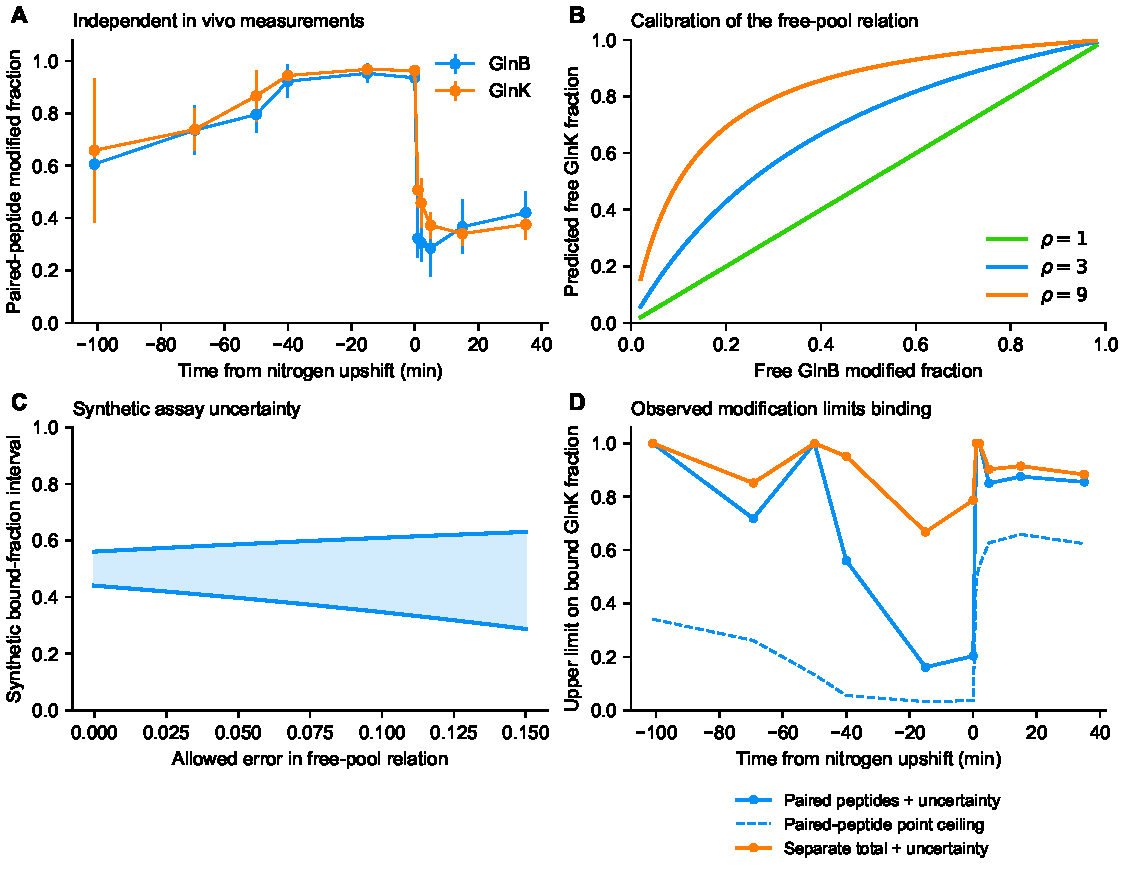
\includegraphics[width=\textwidth,height=0.59\textheight,keepaspectratio]{figure_inputs/paired_paralog_original.pdf}
\caption{\textbf{Paired paralogs motivate a calibrated sequestration assay.} (A) Published wild-type paired-peptide fractions around nitrogen upshift; error bars are conservative first-order SE bounds with unknown covariance. Connecting lines do not establish steady state. (B) Conditional free-pool relation at three relative-specificity values. (C) Synthetic bound-fraction intervals with the control and assay ranges in S1 Appendix A13, allowing an additional absolute error in the free-pool relation. Shading is an admissible interval, not a confidence band. (D) Upper bounds $s_K\leq1-q_K$ on the bound GlnK protein fraction. This is also a bound-trimer fraction for homotrimers; it does not identify mixed-particle counts. The dashed curve uses paired-peptide point fractions; solid curves use working Bonferroni-adjusted $t$ intervals for three component means at each time point, under paired-peptide or separate-total normalization. They do not have established simultaneous coverage across the time course and do not include calibration bias. These ceilings require no stationarity; the calibrated reconstruction in B--C does. None of the curves is a measured bound fraction.}
\end{figure}
\end{document}
